\section{Evaluation}
\subsection{Prüfung der Anforderungen}

\subsubsection{Anforderung 1}
\subsubsection{Anforderung 2}

\subsection{Angriff durch Miner}

Wirtschaftlichkeitsrechnung. Wie hoch muss Potbetrag und Blockreward sind, damit sich dies statistisch lohnt?




\subsection{Aufruf der Auszahlungstransaktion}
Wie bereits in Abschnitt \ref{eth_konzept} betrachtet, ist der Aufruf deiner Funktion zur Auszahlung unumgänglich. Da der Smart Contract dies nicht selber kann, muss der Aufruf entweder von außerhalb oder von einem Anderen Smart Contract kommen.

a) Aufruf von außerhalb:\\
Der Aufruf kann wie in der Implementierung vom Gewinner ausgeführt werden. In diesem Fall zahlt der Gewinner die Transaktionsgebühr und erhält den gesamten Topf-Betrag. Der Gewinner ist dafür zuständig die Funktion rechtzeitig aufzurufen, da der Gewinn sonst in den nächsten Topf übergeht. Eine andere Möglichkeit ist es, dass die Glücksspielanwendung den Smart Contract überwacht und die \textit{payout} Funktion rechtzeitig aufruft. In diesem Fall müsste die Transaktionsgebühr von der Glücksspielanwendung gezahlt werden oder Funktionalität in den Smart Contract eingebaut werden, die die Transaktionskosten vom Topf-Betrag abzieht und der Glücksspielanwendung zurückerstattet. Allerdings verlässt sich der Gewinner dann auf die Anwendung und geht dadurch ein Risiko ein.

b) Aufruf durch Smart Contract:\\
Man kann in der Theorie den Ansatz des Ethereum Alarm Clock \footnote{\url{http://www.ethereum-alarm-clock.com/}} Contracts \footnote{\url{https://etherscan.io/address/0x6c8f2a135f6ed072de4503bd7c4999a1a17f824b}} verwenden, um eine gewünschte Smart Contract Funktion zu einem späteren Zeitpunkt auszuführen. Man spezifiziert dazu welche Funktion man wann (in welchem Blockzeitraum) ausführen möchte und zahlt für die anfallenden Transaktionsgebühren im Voraus. Dies erlaubt, dass eine ganze Reihe von Funktionen sich bei dem Alarm Clock Contract registrieren. Wird nun der Alarm Clock Contract von einem durch einen privaten Schlüssel kontrollierten Account ausgelöst, werden alle registrierten Funktionen aufgerufen. Leider liefert diese Vorgehensweise keine  Garantie, da eine registrierte Funktion nur aufgerufen wird, falls der Alarm Clock Contract aufgerufen wird. Die Glücksspielanwendung müsste also einspringen, sobald niemand anderes bereit ist den Alarm Clock Contract anzustoßen. Es handelt sich also lediglich um eine Vorgehensweise um Transaktionsgebühren mit anderen Ethereum Nutzern zu teilen.

\subsection{Verteilung der Hashfunktion Keccak-256}

Ethereum verwendet die kryptographische Hashfunktion Keccak-256.
Die folgende Monte-Carlo-Simulation zeigt, dass die Hashwerte der Hashfunktion Keccak-256 gleichverteilt sind.
\begin{verbatim}
h=Keccak-256 n=1000000
for i 1 -> n
    hash = h(i);
    result[uint(hash)%10]++
\end{verbatim}
\begin{minipage}{0.5\textwidth}
\begin{verbatim}
Ausgabe:
result[0] =  99227
result[1] = 100479
result[2] = 100163
result[3] =  99804
result[4] =  99945
result[5] = 100208
result[6] = 100403
result[7] = 100438
result[8] = 100035
result[9] =  99298
\end{verbatim}
\end{minipage}
\begin{minipage}{0.5\textwidth}
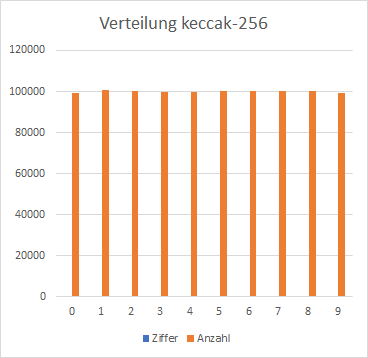
\includegraphics[width=\textwidth]{Figures/verteilung_keccak256}
\centering
\decoRule
\captionof{figure}{Verteilung der Keccak-256 Hashfunktion}
\label{fig:verteilung_keccak256}
\end{minipage}

\subsection{Sicherheit von Smart Contracts}
Hier dann die DAO erwähnen und die Probleme erklären. Und am Beispiel unseres Smart Contracts aufzeigen. 

Hier dann noch darauf eingehen, dass man auf keinen Fall bock.timestamp verwenden sollte, da Miner auf diesen einen direkten Zugriff haben können.

https://ethereum.stackexchange.com/questions/19341/address-send-vs-address-transfer-best-practice-usage

Hier dann nur darauf eingehen, dass falls man die Auszahlung mittels der unsicheren Methode macht ein BUG besteht. 

Anscheinend ist bei address.transfer aber sicher, dass kein contract code ausgeführt wird. Es gibt allerdings 3 Möglichkeiten zu senden.
Eine ist unsicher.

\begin{lstlisting}[basicstyle=\small]
function payout() public{
    assert(potClosed);
    assert(block.number>payoutBlockNumber);
    potClosed = false; //fixes bug
    payoutBlockHash = block.blockhash(payoutBlockNumber); 
    if(payoutBlockHash == 0){
        nbrOfMissedPayouts++;
    }else{
        winner = uint(payoutBlockHash) % NBR_OF_SLOTS;
        address winnerAddress = payoutAddresses[winner];
        uint amount= EXPECTED_POT_AMOUNT*NBR_OF_SLOTS;
        amount += EXPECTED_POT_AMOUNT*NBR_OF_SLOTS*nbrOfMissedPayouts;
        winnerAddress.transfer(amount); // send pot amount to winner
        nbrOfMissedPayouts = 0;
    }
    nbrOfParticipants=0;
}
\end{lstlisting}



Die Solidity Dokumentation \footnote{\url{https://solidity.readthedocs.io/en/develop/security-considerations.html}} listet eine Reihe von Beispielen, die die Sicherheit von Smart Contracts betreffen. Entwickler sollten sich dieser bewusst sein, bevor sie einen Smart Contract veröffentlichen der Geld verwaltet.

\subsubsection{Problembeschreibung}
Code öffentlich, Bugs nicht fixbar.
\subsubsection{Beispiel}
Gambling Smart Contract mit Bug